\documentclass[12pt]{article}
\usepackage[utf8]{inputenc}
\usepackage[T1]{fontenc}
\usepackage{lmodern}
\usepackage[margin=2.54cm]{geometry}
\usepackage[provide=*]{babel}
\babelprovide[import,main]{french}
\usepackage{amsmath,amssymb}
\usepackage{graphicx}
\usepackage{tabularx}
\usepackage{longtable}
\usepackage{booktabs}
\usepackage{array}
\usepackage{url}
\usepackage{hyperref}

\setlength\parindent{0pt}
\setlength\parskip{0.5em}

\title{Projet 1 -- Plateforme de priorisation des vulnérabilités IoT\\
\large 8INF917 -- Sécurité informatique pour l'Internet des Objets}
\author{Arno Bidet \and Célian Bellenge \and Joseph Balsan \and Martial Fousset}
\date{9 mars 2026}

\begin{document}

\maketitle

\begin{abstract}
Ce rapport présente la conception, l'implémentation et l'évaluation d'une plateforme web de priorisation des vulnérabilités pour un parc de caméras IP. L'application consolide des données ouvertes (NVD/CVE, CISA KEV, CWE et EPSS), les relie aux équipements suivis par l'utilisateur, puis restitue des indicateurs exploitables: score CVSS agrégé, statut de risque par actif, niveau d'exploitation connue (KEV), recommandations de mitigation et filtres d'analyse. La solution est volontairement défensive, reproductible via Docker Compose et orientée prise de décision opérationnelle (patching, segmentation réseau, durcissement des configurations et priorisation des actions). Le document détaille l'architecture, le pipeline de collecte, le modèle de données, la méthode de priorisation, les résultats observés, les limites actuelles et les pistes d'amélioration.
\end{abstract}

\tableofcontents
\newpage

\section{Introduction et contexte}
La surface d'attaque des objets connectés augmente à mesure que les équipements en périphérie de réseau se multiplient. Les caméras IP, les routeurs, les passerelles et les capteurs sont souvent déployés rapidement, avec des configurations hétérogènes et des cycles de mise à jour irréguliers. Dans ce contexte, les équipes techniques doivent faire face à un volume de vulnérabilités difficile à absorber, à une visibilité imparfaite sur les vulnérabilités effectivement exploitées, et à une difficulté récurrente de priorisation lorsqu'il faut arbitrer entre correction immédiate, mitigation temporaire et dette de sécurité.

Ce projet répond à ce besoin en proposant une plateforme web orientée priorisation. L'objectif n'est pas d'afficher un simple inventaire de CVE, mais d'aider à décider quelles vulnérabilités traiter en priorité selon la sévérité technique, la probabilité d'exploitation et le contexte de criticité métier des actifs concernés. La solution s'appuie uniquement sur des sources ouvertes et gratuites, dans un cadre strictement défensif.

\section{Objectifs du projet et périmètre}
Le périmètre retenu couvre la famille des caméras IP en contexte domestique et PME, avec une base d'exemples multi-vendeurs incluant notamment Hikvision, Dahua, Axis, Amcrest, Reolink et Bosch. Le projet vise à collecter automatiquement des vulnérabilités publiques, à les enrichir avec des signaux de priorisation, puis à proposer une restitution exploitable par un utilisateur non spécialiste. Le système doit rester compréhensible, reproductible et défensif. En particulier, il n'implique ni scan Internet, ni test d'intrusion, ni publication de techniques offensives.

Sur le plan fonctionnel, la plateforme doit relier des CVE à des équipements suivis, intégrer des métriques de risque complémentaires au CVSS, offrir des filtres d'analyse et produire des recommandations concrètes de mitigation. Le résultat attendu est une aide à la décision opérationnelle, pas un moteur d'attaque ni un outil de preuve de concept offensive.

\section{Architecture générale}
La plateforme est organisée autour de trois composants. Le premier composant est l'application Next.js en TypeScript, qui gère l'interface, l'authentification, les opérations CRUD sur les caméras et les vues d'analyse. Le deuxième composant est un microservice Python chargé de la synchronisation des renseignements de vulnérabilités et de plusieurs agrégations de risque. Le troisième composant est une base PostgreSQL qui centralise les entités utilisateurs, caméras, CVE, CWE, KEV, EPSS et les tables de liaison entre ces éléments. L'orchestration est réalisée avec Docker Compose, ce qui permet un déploiement local reproductible et homogène.

Cette séparation est volontaire. Elle permet de maintenir une interface web stable tout en faisant évoluer la logique de collecte et d'analyse dans le microservice Python. Elle facilite aussi les tests et l'isolement des responsabilités. Côté application web, les pages principales sont la vue d'ensemble, l'analyse des menaces, la gestion des caméras et le détail d'une caméra. Côté API, la plateforme expose des routes d'authentification, de gestion des caméras et de consultation des vulnérabilités. Côté service Python, des endpoints dédiés permettent de synchroniser les données et d'exposer des synthèses orientées tableau de bord.

La vue d'architecture globale est présentée en figure~\ref{fig:architecture_globale}. Elle illustre les flux entre l'interface Next.js, le microservice Python, la base PostgreSQL et les sources externes.

\begin{figure}[htbp]
\centering
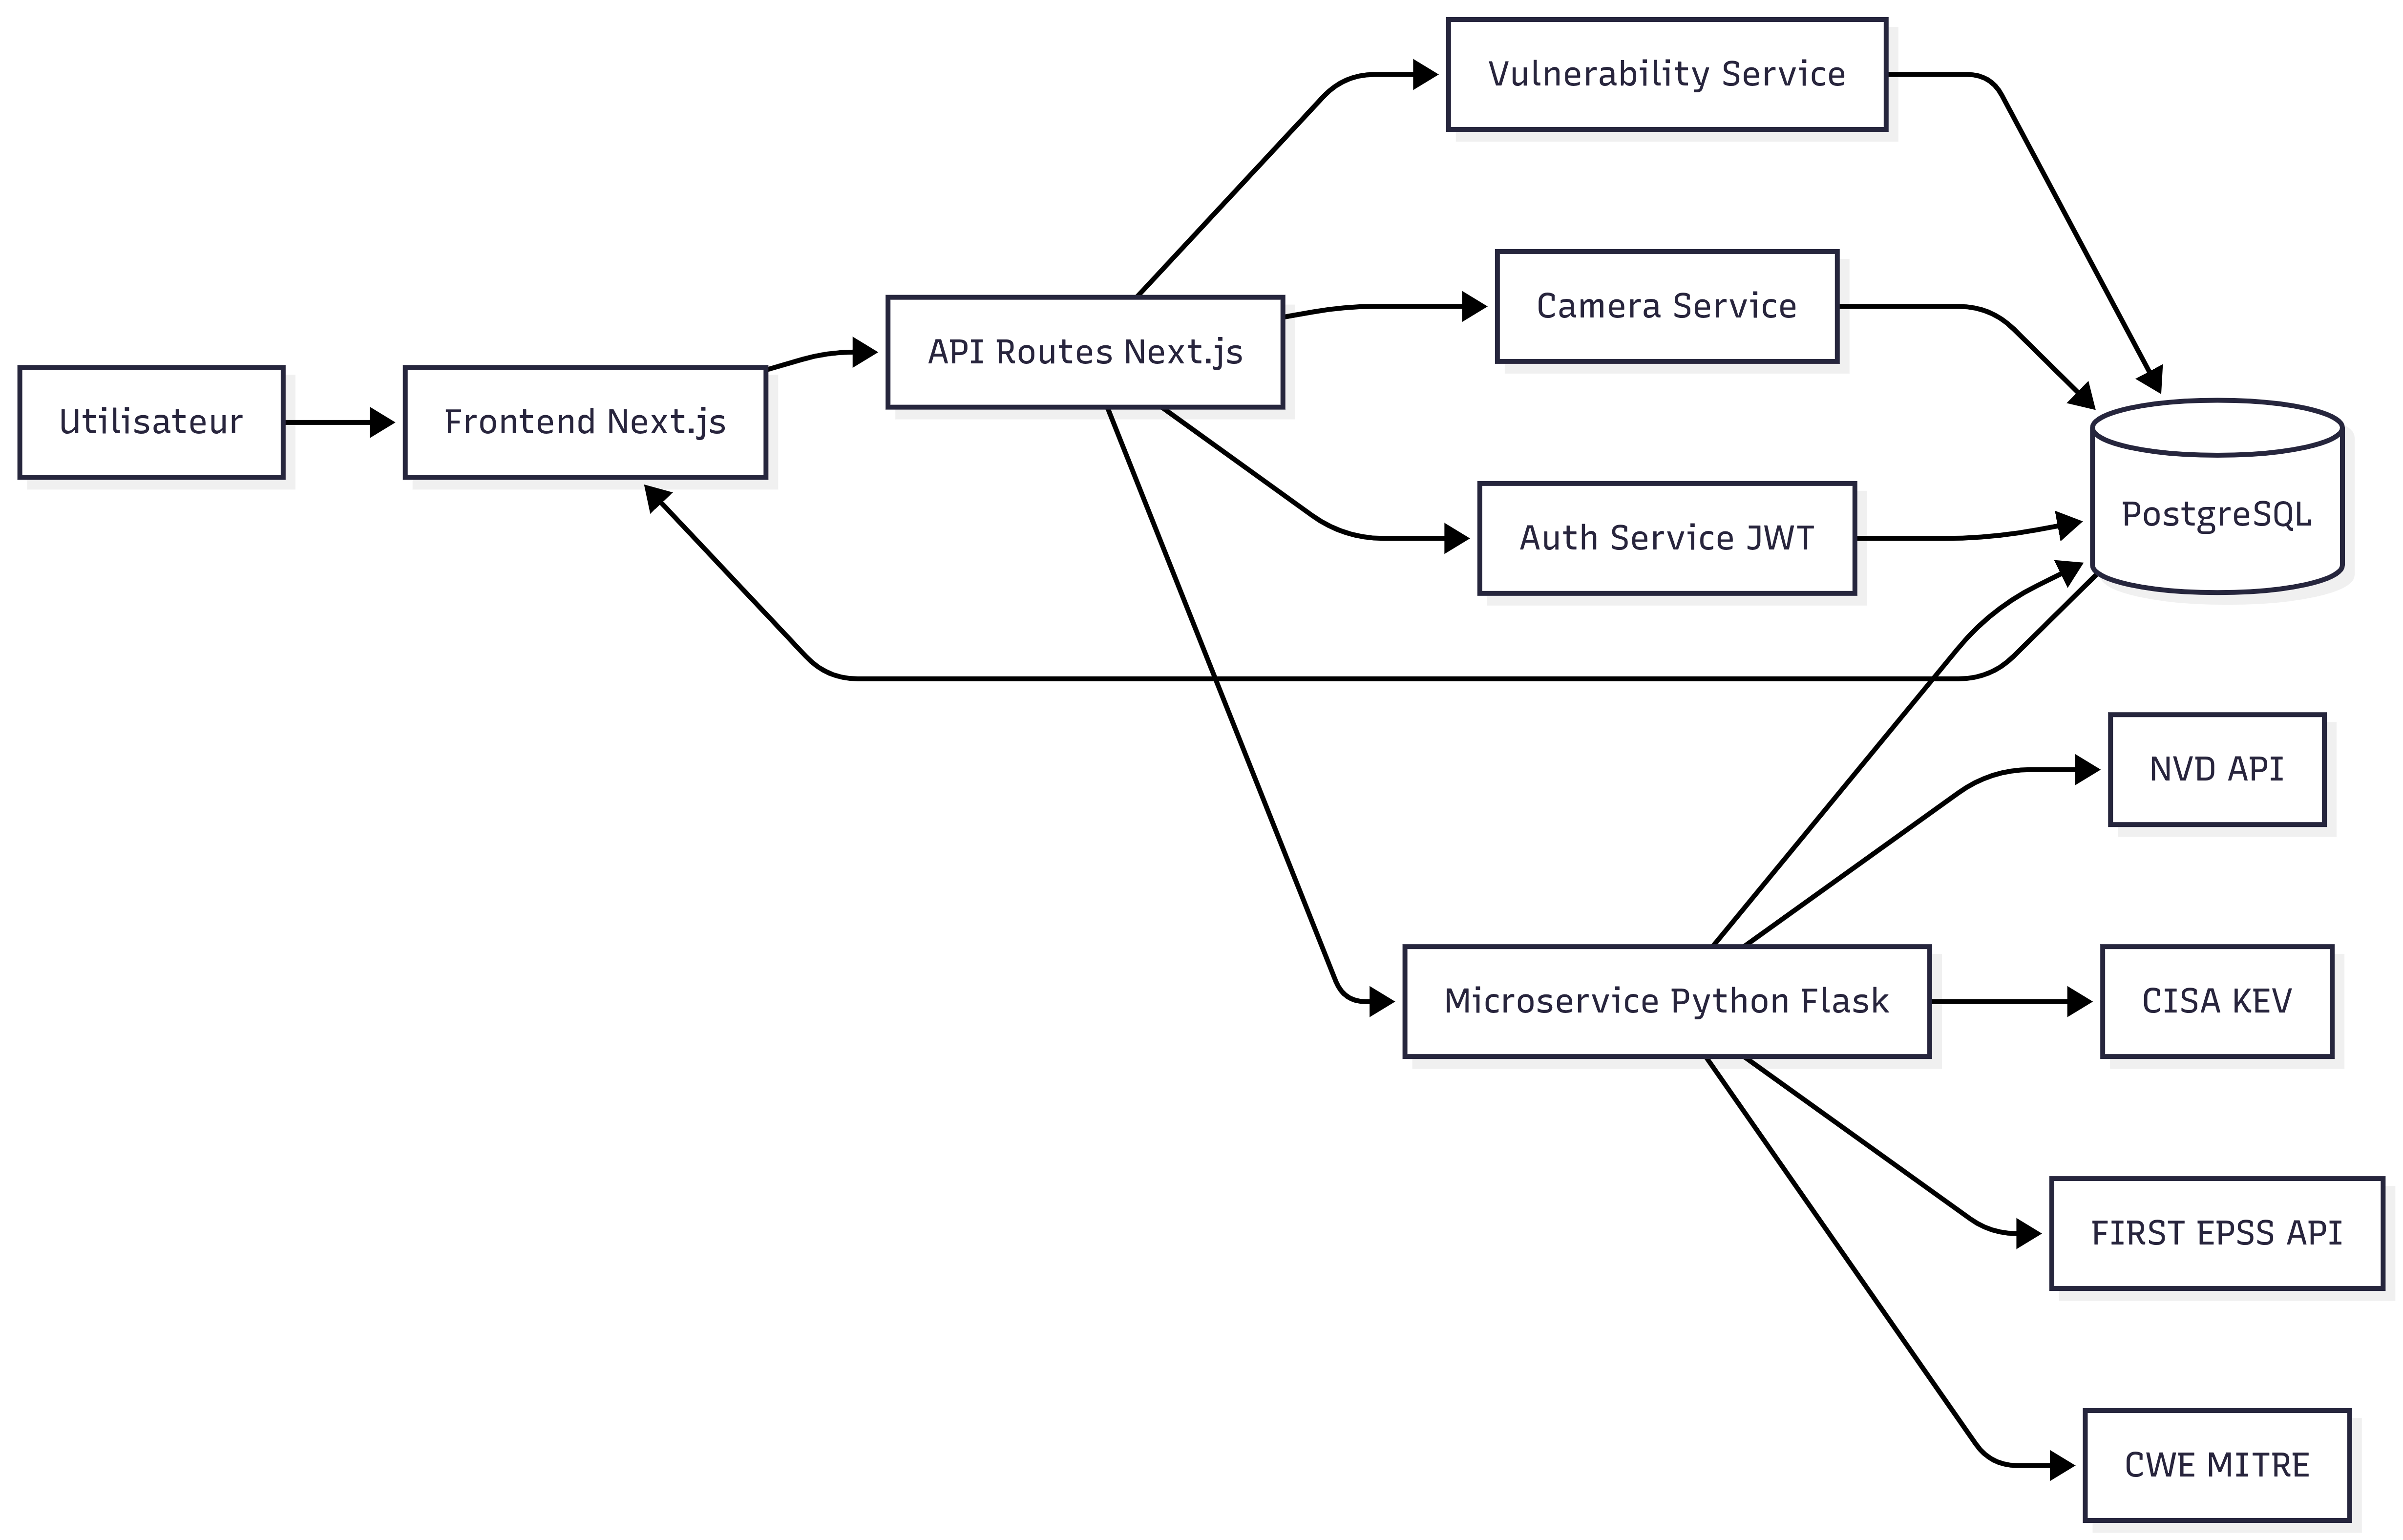
\includegraphics[width=0.92\textwidth,height=0.38\textheight,keepaspectratio]{img/fig01_architecture_globale.png}
\caption{Architecture globale de la plateforme de priorisation IoT.}
\label{fig:architecture_globale}
\end{figure}

\section{Pipeline de collecte et d'enrichissement}
Le pipeline de collecte commence par l'ingestion des vulnérabilités via les flux publics NVD. Les CVE récupérées sont normalisées puis insérées en base. Un appariement est ensuite réalisé entre les modèles de caméras et les CVE au moyen des informations de fournisseur et de produit, puis stocké dans des tables de liaison. Les CVE sont enrichies avec l'information KEV pour signaler les vulnérabilités activement exploitées, puis avec EPSS pour estimer la probabilité d'exploitation. Les entrées CWE sont également exploitées afin d'améliorer la compréhension du type de faiblesse et de nourrir la génération de recommandations.

La synchronisation peut être déclenchée explicitement par endpoint, mais elle est aussi sollicitée dans certains scénarios de consultation pour rafraîchir les données de manière opportuniste. Ce compromis entre fraîcheur et coût d'appel API évite de lancer des mises à jour lourdes en continu tout en maintenant une pertinence suffisante des résultats affichés.

La résilience du pipeline repose sur des mécanismes simples mais efficaces: retours de repli cohérents lorsque les services externes sont indisponibles, intégrité relationnelle en base, déduplication des associations grâce aux clés composites et limitation de la volumétrie affichée dans l'interface pour conserver de bonnes performances.

Le déroulement détaillé du pipeline de collecte et d'enrichissement est donné en figure~\ref{fig:pipeline_collecte}. Ce schéma met en évidence l'enchaînement NVD $\rightarrow$ normalisation $\rightarrow$ enrichissement KEV/EPSS/CWE $\rightarrow$ agrégation et restitution.

\begin{figure}[htbp]
\centering
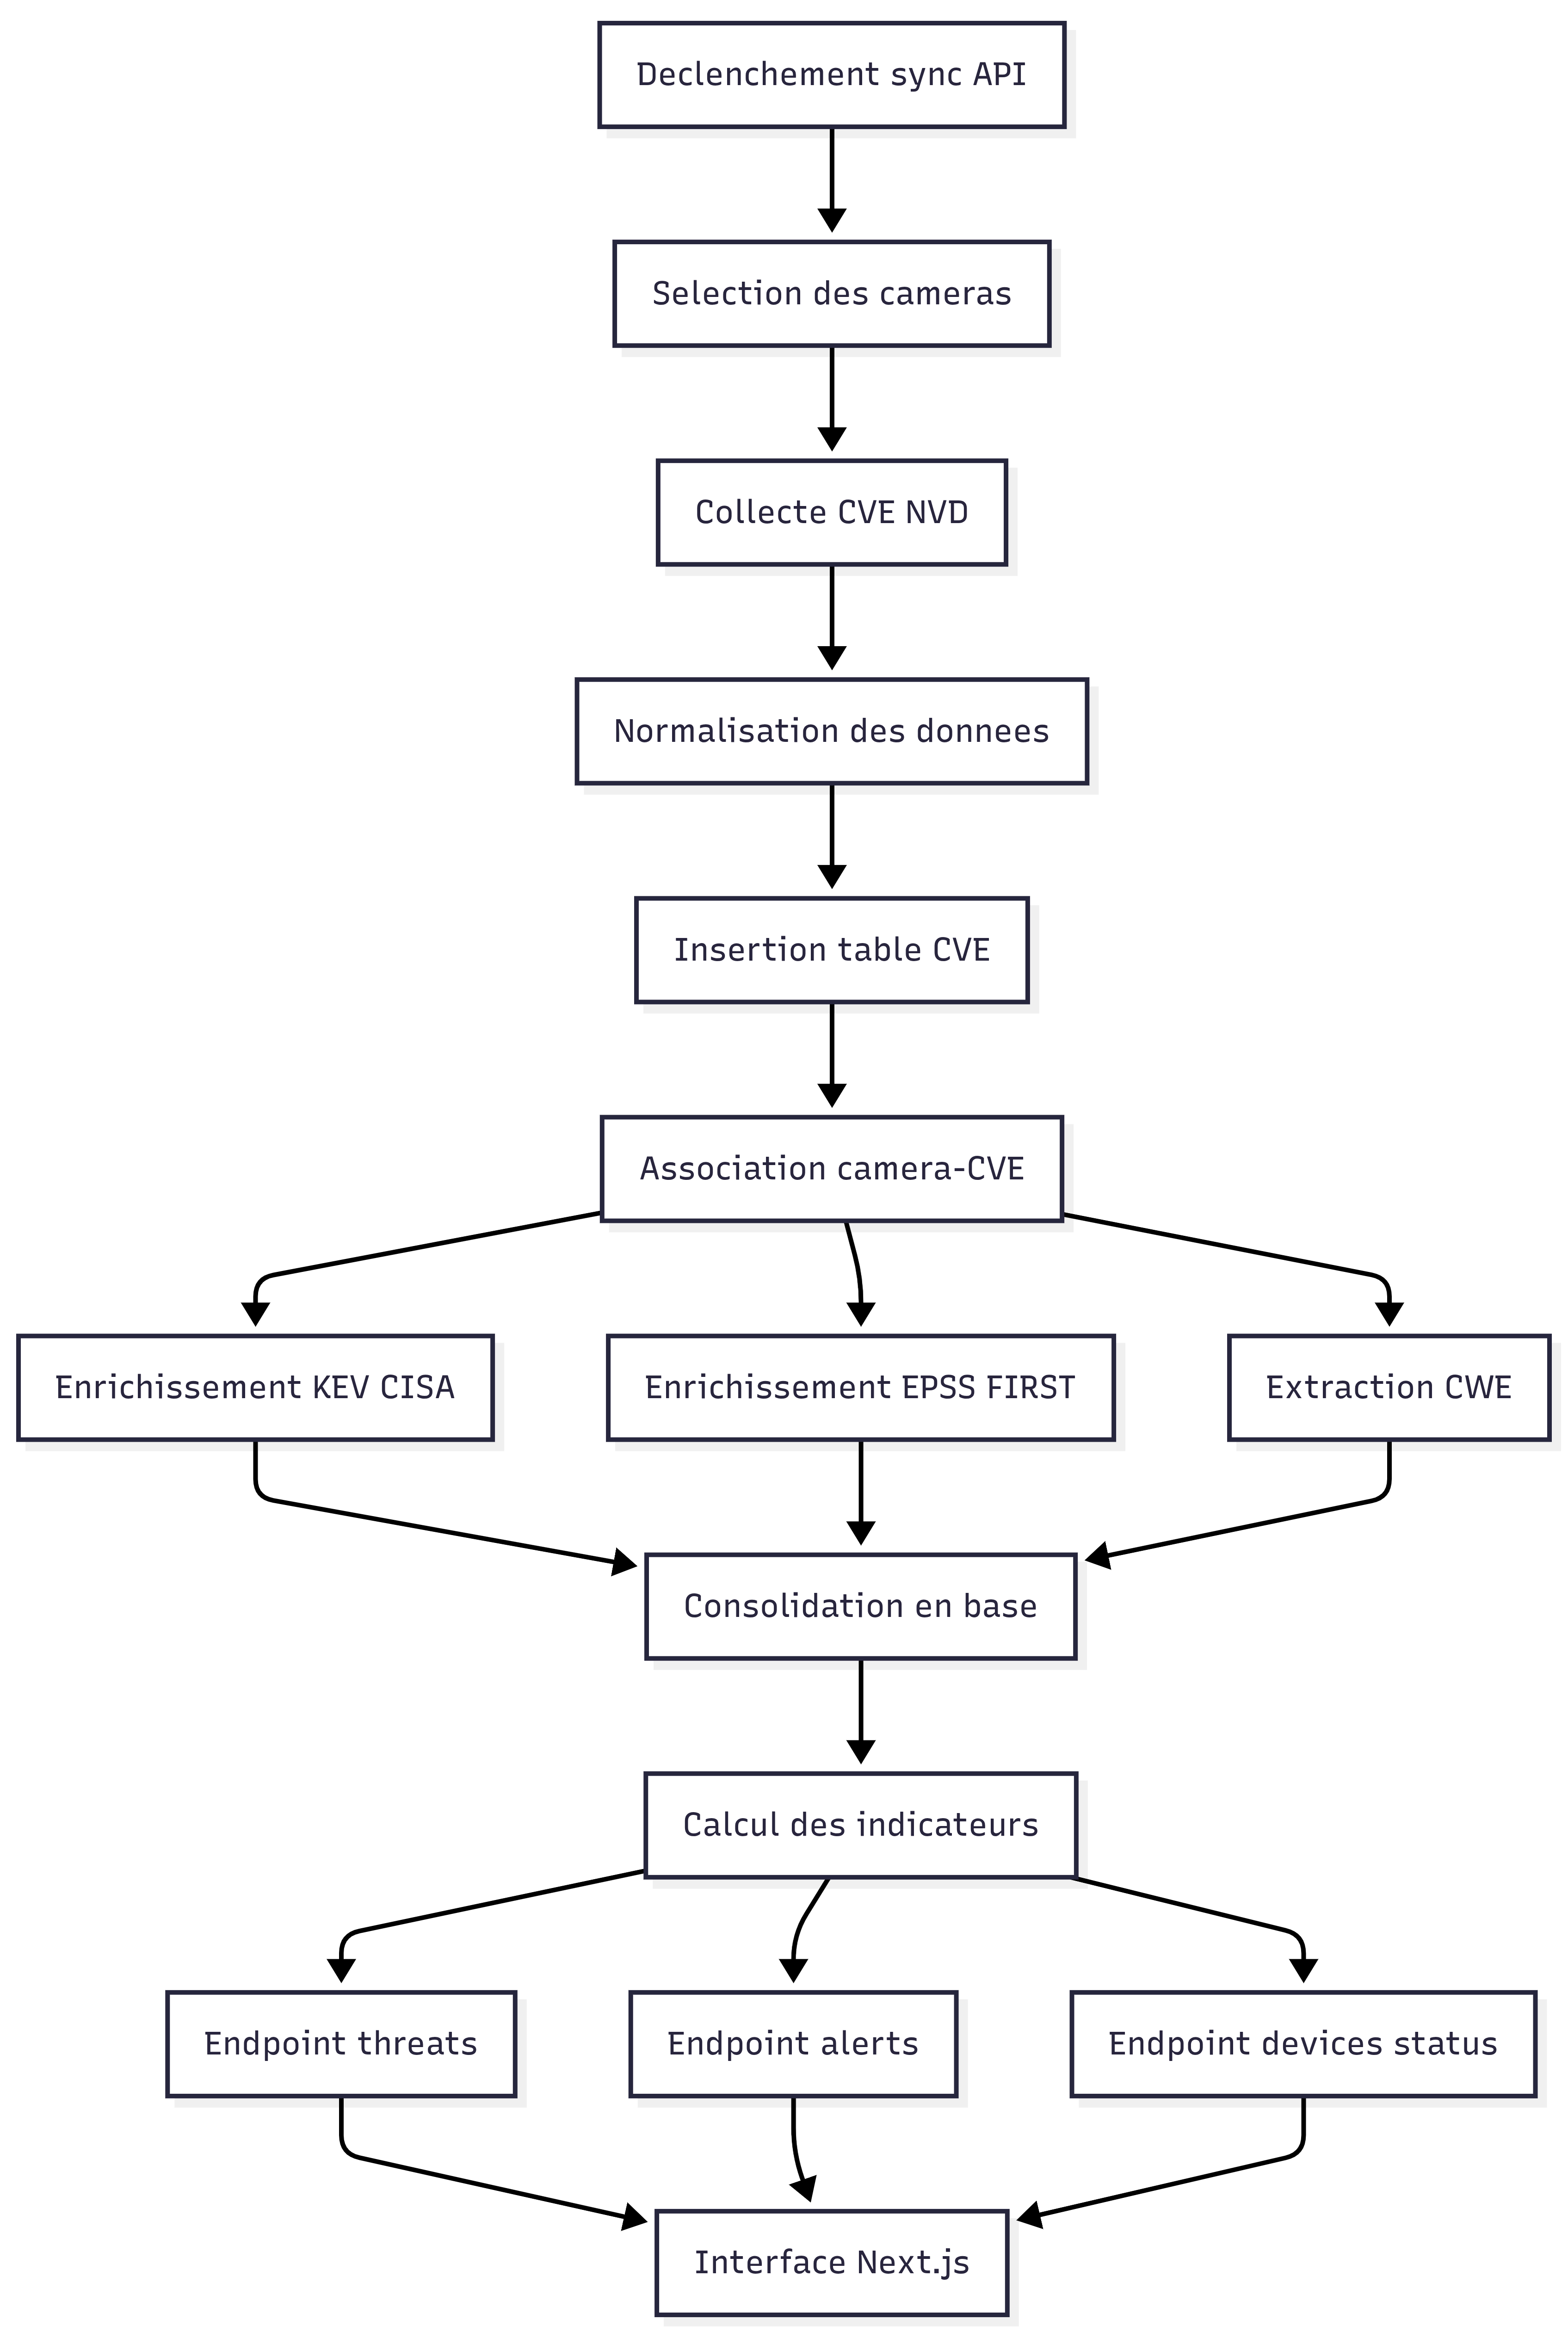
\includegraphics[width=0.92\textwidth,height=0.38\textheight,keepaspectratio]{img/fig02_pipeline_collecte_enrichissement.png}
\caption{Pipeline de collecte, enrichissement et publication des indicateurs.}
\label{fig:pipeline_collecte}
\end{figure}

\section{Modèle de données}
Le modèle relationnel est centré sur les tables \texttt{users}, \texttt{cameras} et \texttt{cves}, complétées par \texttt{kev}, \texttt{epss}, \texttt{cwes} et plusieurs tables d'association. La table \texttt{cameras} contient notamment un niveau de criticité métier, indispensable pour contextualiser la priorisation. Les tables \texttt{camera\_cves}, \texttt{camera\_kev} et \texttt{camera\_cwes} permettent de conserver une représentation explicite des liens entre actifs et vulnérabilités.

Cette modélisation évite la redondance et facilite les requêtes analytiques. Les référentiels globaux sont stockés une seule fois, puis reliés aux actifs suivis. Les contraintes d'intégrité et les index ajoutés dans le script d'initialisation garantissent une base robuste pour la restitution en temps raisonnable, même lorsque le nombre de CVE augmente.

Le modèle relationnel simplifié apparaît en figure~\ref{fig:modele_donnees}. Les cardinalités principales montrent comment une caméra peut être liée à plusieurs CVE, et comment ces CVE sont ensuite enrichies par KEV, EPSS et CWE.

\begin{figure}[htbp]
\centering
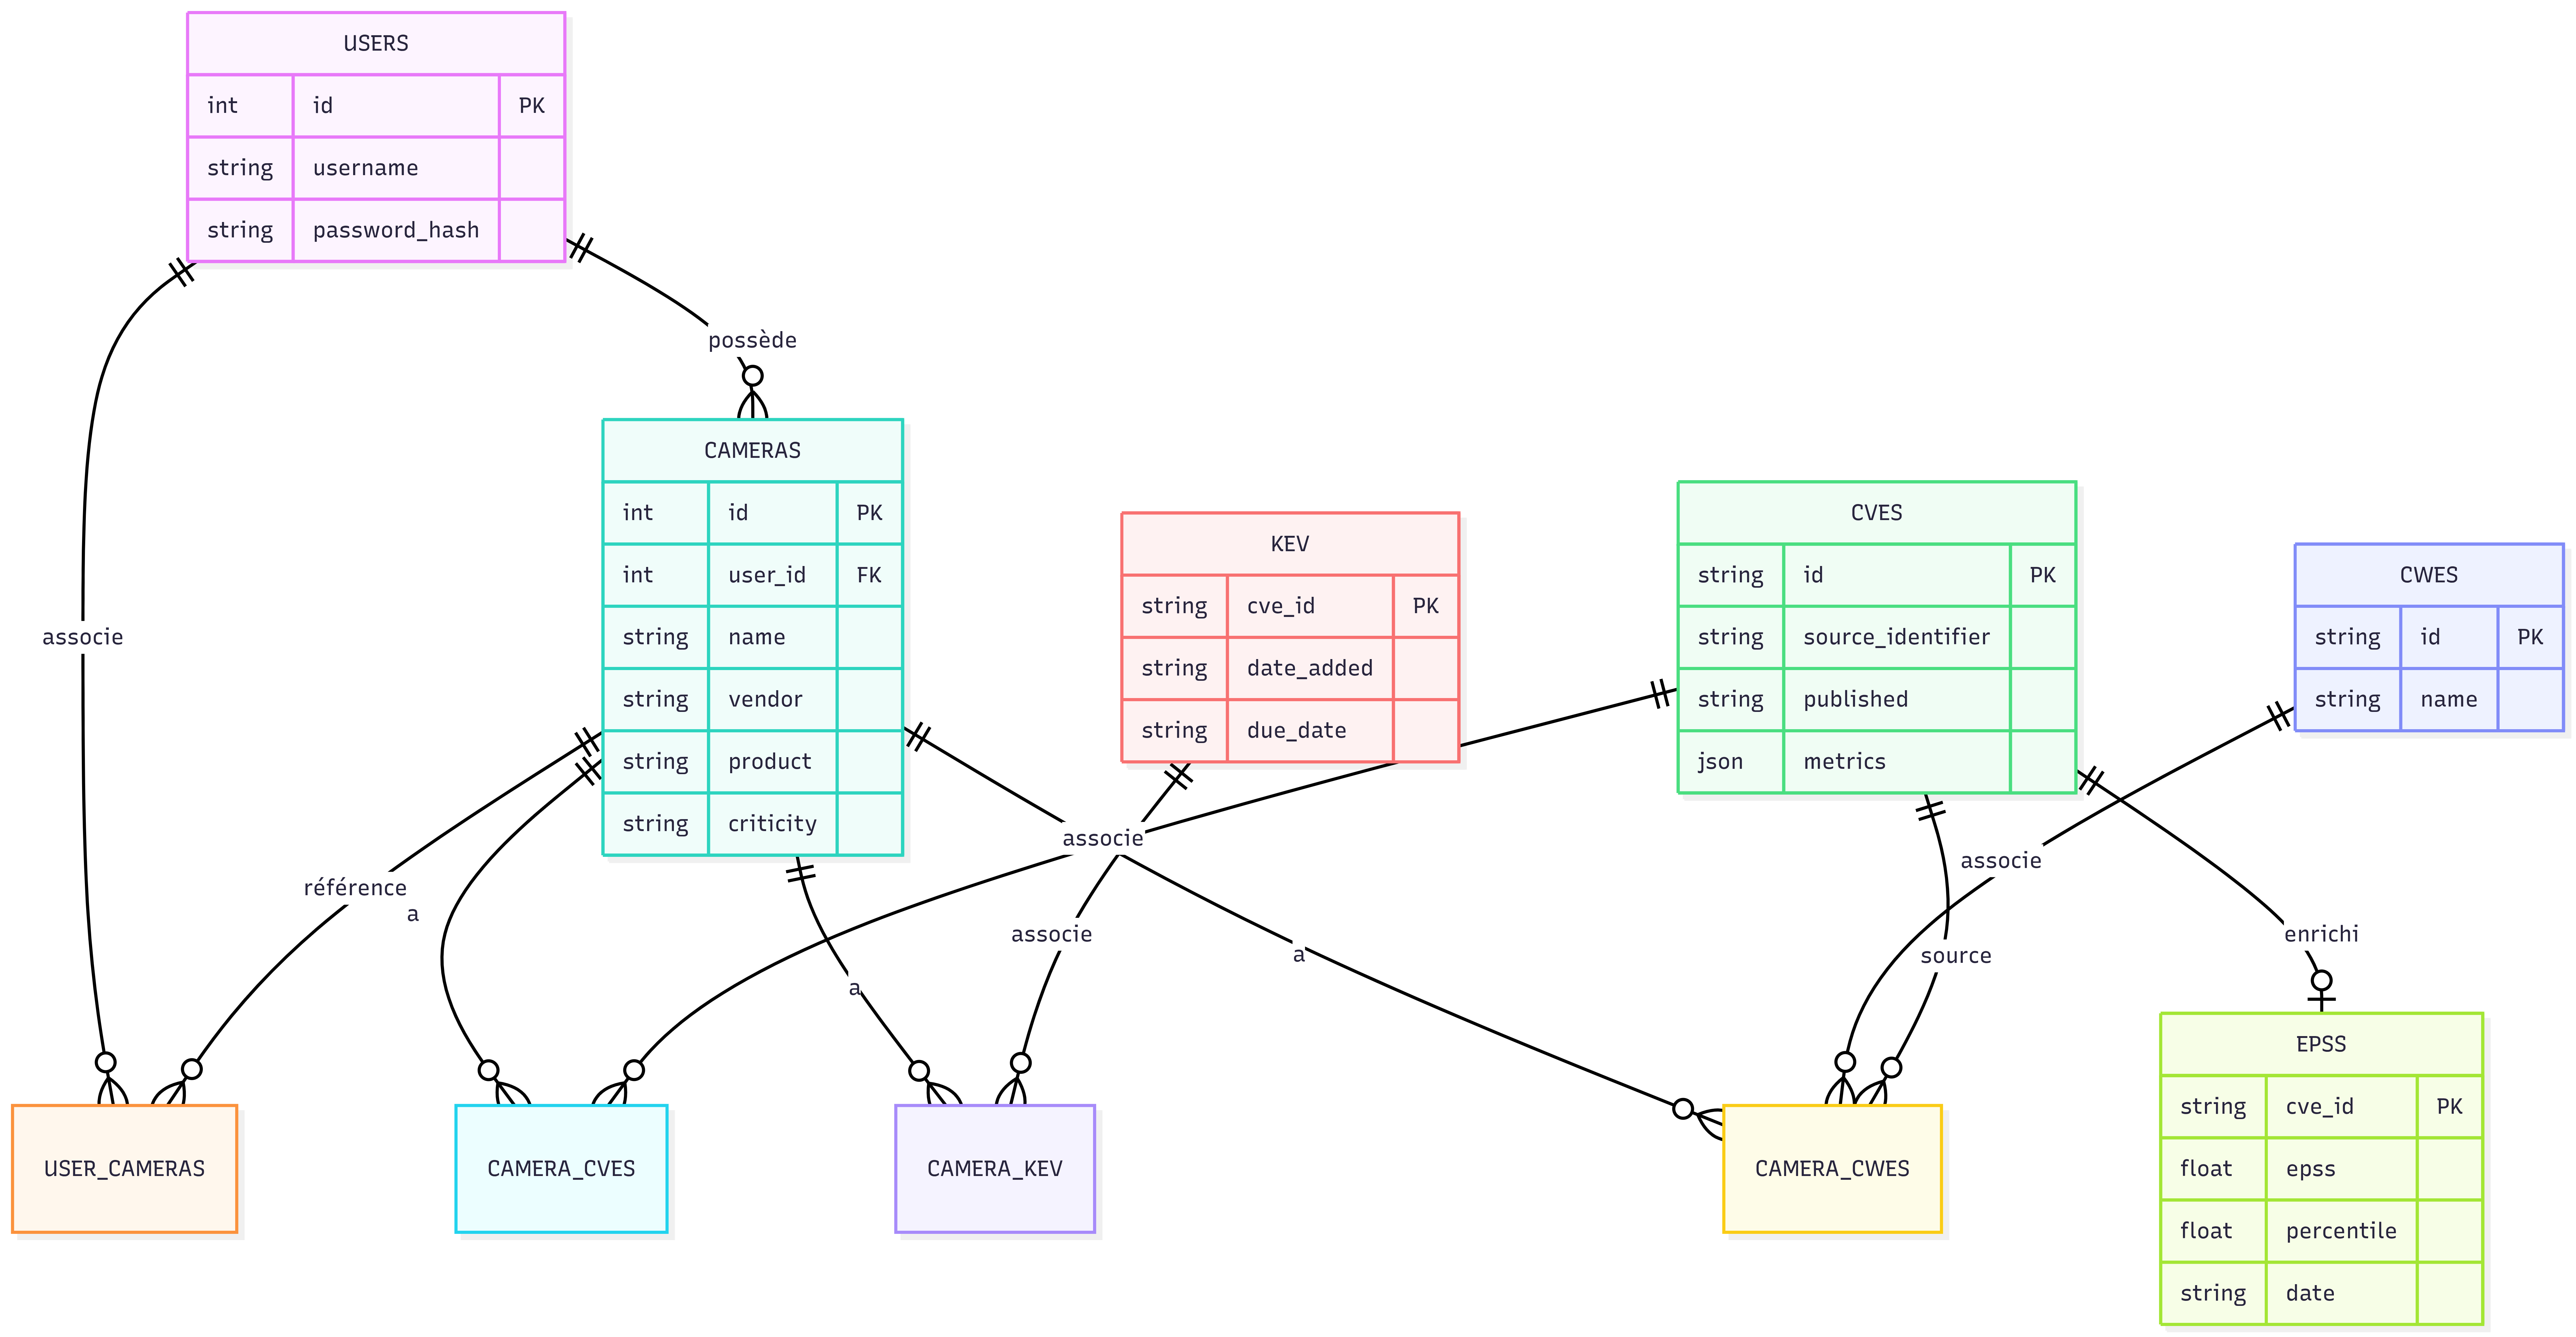
\includegraphics[width=0.92\textwidth,height=0.38\textheight,keepaspectratio]{img/fig03_modele_donnees_relationnel.png}
\caption{Modèle de données relationnel simplifié.}
\label{fig:modele_donnees}
\end{figure}

\section{Méthode de priorisation du risque}
Conformément aux consignes, la priorisation ne repose pas uniquement sur le CVSS. Le projet combine l'impact technique, l'information d'exploitation observée et la probabilité d'exploitation. Cette combinaison est réalisée dans le module Python de manière explicable, afin de garder une transparence totale sur les critères de classement.

Le calcul du score de risque CVE est défini par la formule suivante:
\[
\text{Risk}_{CVE} = 100 \times \left(0.6\times\frac{CVSS}{10} + 0.3\times EPSS + 0.1\times KEV\right)
\]

La variable $KEV$ vaut 1 lorsque la CVE appartient au catalogue CISA des vulnérabilités exploitées, sinon 0. Une majoration supplémentaire est appliquée en présence d'indicateurs associés à des campagnes ransomware. Le score appareil est ensuite construit à partir des vulnérabilités les plus critiques pour éviter qu'un grand nombre de vulnérabilités faibles masque un petit nombre de vulnérabilités très dangereuses.

Le score de risque d'un appareil est calculé selon:
\[
\text{Risk}_{device} = 0.6\times\max(\text{top-5}) + 0.4\times\text{moyenne}(\text{top-5})
\]

Dans l'interface Next.js, un statut opérationnel \texttt{secure}, \texttt{warning} ou \texttt{vulnerable} est dérivé du CVSS moyen, corrigé par un multiplicateur de criticité métier. Ce multiplicateur est de 0.5 pour \texttt{low}, 1.0 pour \texttt{medium}, 1.5 pour \texttt{high} et 2.0 pour \texttt{critical}. Cette stratégie permet de tenir compte de l'importance métier de l'actif tout en conservant un lien direct avec les métriques de sécurité.

La logique de priorisation complète est synthétisée en figure~\ref{fig:priorisation_risque}, depuis les métriques brutes jusqu'aux recommandations classées en priorité.

\begin{figure}[htbp]
\centering
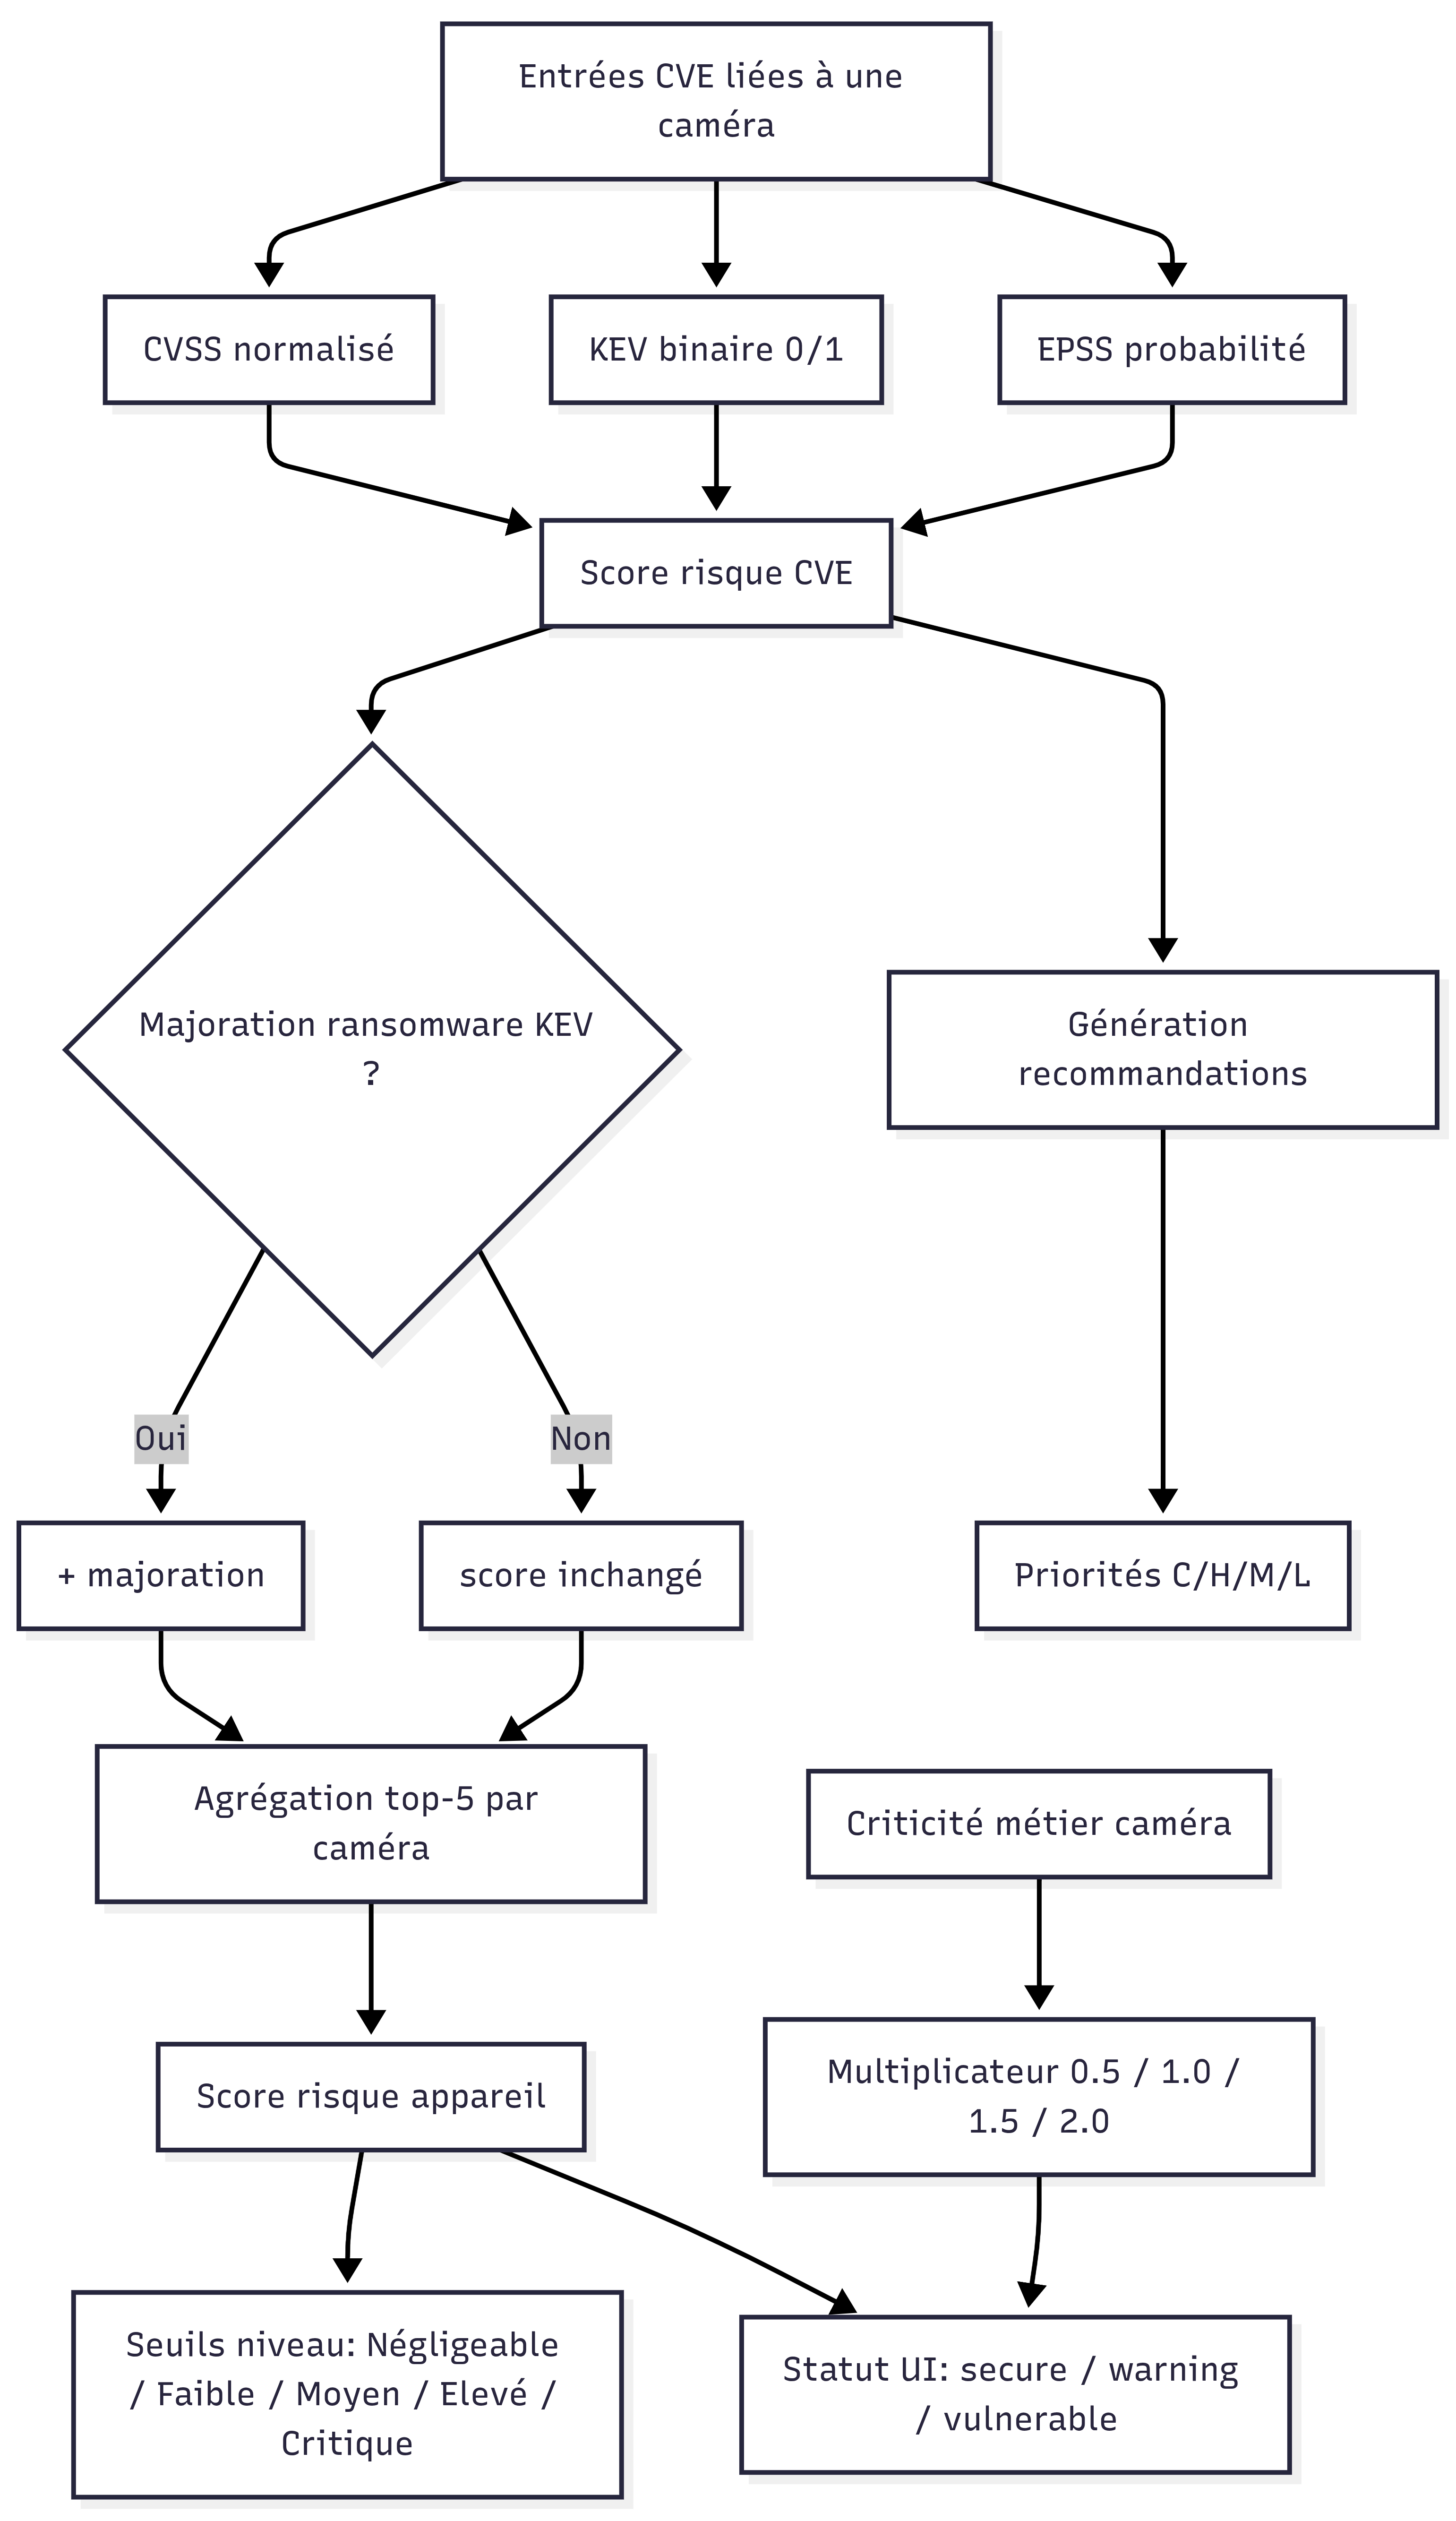
\includegraphics[width=0.92\textwidth,height=0.38\textheight,keepaspectratio]{img/fig04_methode_priorisation_risque.png}
\caption{Chaîne de calcul de la priorisation du risque et restitution.}
\label{fig:priorisation_risque}
\end{figure}

\section{Interface web et fonctionnalités livrées}
La plateforme couvre les attendus du MVP. Le module de collecte est opérationnel, le stockage est structuré en base relationnelle, la priorisation est explicite et les vues front permettent une consultation détaillée des résultats. La page de gestion des caméras propose la création, la modification et la suppression d'actifs avec affectation d'une criticité métier. La page d'analyse des menaces affiche les alertes et l'historique, avec des filtres sur la sévérité, la catégorie, le statut de résolution, le type et la source. La page de détail caméra expose les indicateurs agrégés, la liste des CVE, des CWE et des entrées KEV, avec des filtres de recherche, de sévérité et d'état KEV.

Les recommandations sont générées à partir de règles simples construites sur les niveaux CVSS, les familles CWE et la criticité de l'actif. Elles sont ensuite normalisées en objets contenant un titre, une description et une priorité. Dans l'interface, les lettres C, H, M et L correspondent aux priorités Critical, High, Medium et Low. Ce choix de représentation compacte a été retenu pour rendre la lecture rapide dans les cartes de recommandations.

\section{Sécurité, conformité et posture défensive}
Le projet respecte une posture strictement défensive. L'application n'exécute aucune activité intrusive, ne réalise aucun scan d'Internet et n'embarque aucun contenu d'exploitation. Les seules données consommées proviennent de sources publiques, gratuites et documentées. L'authentification est assurée côté application via jeton en cookie HTTP-only, et la séparation entre la couche web et la couche de synchronisation réduit l'exposition des composants internes.

Du point de vue de la confidentialité, la plateforme manipule un volume restreint de données personnelles, essentiellement liées aux comptes et aux inventaires d'équipements. La conception favorise la minimisation des données, l'isolation des responsabilités et la traçabilité des origines de données externes. Cette approche s'inscrit dans les bonnes pratiques attendues pour un projet académique orienté sécurité défensive.

\section{Résultats, discussion et limites}
Le prototype produit une chaîne fonctionnelle de bout en bout. L'intégration NVD, KEV, EPSS et CWE est effective, les associations avec les caméras sont persistées en base, la priorisation est calculée et les vues front permettent une restitution lisible. La reproductibilité est validée par l'exécution conteneurisée, ce qui facilite la démonstration en environnement de présentation.

Certaines limites doivent toutefois être soulignées. L'appariement vendor/product peut générer des faux positifs lorsque les métadonnées sont ambiguës. Les descriptions CVE sont inégales selon les éditeurs, ce qui affecte parfois la qualité des recommandations. L'intégration d'EPSS est solide côté collecte et calcul, mais la restitution pourrait encore être harmonisée sur toutes les vues de l'interface. Enfin, la dépendance aux quotas et à la disponibilité des API externes impose des mécanismes de cache et de planification plus avancés pour une exploitation continue à grande échelle.

Malgré ces limites, la méthode retenue est pertinente pour un cadre académique. Elle reste explicable, traçable et suffisamment robuste pour démontrer la valeur d'une priorisation multi-critères dans un contexte IoT.

\section{Plan d'amélioration}
Les prochaines itérations viseront d'abord à uniformiser l'exposition du score de risque sur l'ensemble de l'interface, puis à renforcer la fiabilité de l'appariement entre actifs et vulnérabilités. Une piste immédiate consiste à introduire des tests automatiques de non-régression sur les calculs de risque, afin de garantir la stabilité de la priorisation lors des évolutions de code. Il serait également utile d'ajouter des exports exploitables en contexte opérationnel, par exemple en CSV ou PDF, pour faciliter la communication entre équipes techniques et responsables métiers.

À moyen terme, un moteur d'appariement plus robuste avec score de confiance améliorerait la précision des associations. L'historisation des scores permettrait de suivre les tendances de risque et de mesurer les délais de remédiation. Un mécanisme de planification périodique plus élaboré, couplé à une politique de cache, limiterait la dépendance aux appels externes. Enfin, l'extension du périmètre à d'autres familles d'objets connectés renforcerait la portée du projet.

\section{Reproductibilité du projet}
Le projet est reproductible avec Docker Compose, ce qui permet d'initialiser l'ensemble de la pile dans un environnement local cohérent:
\begin{verbatim}
docker compose up --build
\end{verbatim}

Cette commande lance l'interface web Next.js, le microservice Python et la base PostgreSQL initialisée par script SQL. Le dépôt contient également un README détaillant les dépendances, les commandes d'exécution et la structure du projet, ce qui permet à un tiers de reproduire rapidement les résultats présentés dans ce rapport.

\section{Conclusion}
La plateforme livrée répond aux exigences centrales du projet: collecte automatique à partir de sources publiques, enrichissement des CVE avec contexte d'exploitation, priorisation explicite et restitution orientée décision. Le système est défensif, reproductible et extensible. En pratique, l'approche permet de passer d'une logique de liste de vulnérabilités à une logique d'arbitrage du risque: \textit{quoi corriger en premier, sur quel actif, et avec quelle mesure}. Les travaux futurs porteront principalement sur l'amélioration de la qualité d'appariement, la généralisation EPSS dans toutes les vues et l'industrialisation des analyses de tendance.

\newpage
\section*{Références et sources open-source (consultées le 9 mars 2026)}
\addcontentsline{toc}{section}{Références}

Les principales sources utilisées sont la base NVD et sa documentation développeur, le catalogue CISA KEV et ses ressources, la documentation FIRST EPSS et son API, le programme CVE, la taxonomie CWE de MITRE, ainsi que les documents de référence ETSI EN 303 645, NISTIR 8259A et NISTIR 8259B. Les URL sont les suivantes: \url{https://nvd.nist.gov/}, \url{https://nvd.nist.gov/developers/vulnerabilities}, \url{https://www.cisa.gov/known-exploited-vulnerabilities-catalog}, \url{https://www.cisa.gov/resources-tools/resources/kev-catalog}, \url{https://www.first.org/epss/}, \url{https://www.first.org/epss/api}, \url{https://www.cve.org/}, \url{https://cwe.mitre.org/}, \url{https://www.etsi.org/deliver/etsi_en/303600_303699/303645/03.01.03_60/en_303645v030103p.pdf}, \url{https://nvlpubs.nist.gov/nistpubs/ir/2020/NIST.IR.8259a.pdf} et \url{https://nvlpubs.nist.gov/nistpubs/ir/2021/NIST.IR.8259B.pdf}.

\end{document}